% 建议放在词级置信度公式及其解释之后、本小节结尾过渡段之前。
% 将配套PDF放入论文的 figures 目录。

为直观说明由字符路径形成词时间区间的过程，图~\ref{fig:p1_ctc_word_alignment}
展示了样本 \texttt{-egA8-b7-3M\$\_\$1} 中
\texttt{successful Legal} 对应的局部对齐结果。三个子图共用时间轴，
依次呈现原始音频波形、目标字符概率与最优路径选中的位置，以及合并后的词级时间区间。
概率图的纵轴按目标字符在转写中的顺序排列，颜色越深表示对应字符的输出概率越高；
圆点标示完整转写的最优路径在该局部片段中选中的位置，蓝色和橙色分别对应两个词，
灰色对应词界符或空白符。其中，\texttt{|} 表示词界符，空白符单独列于图底部。

\begin{figure}[htbp]
    \centering
    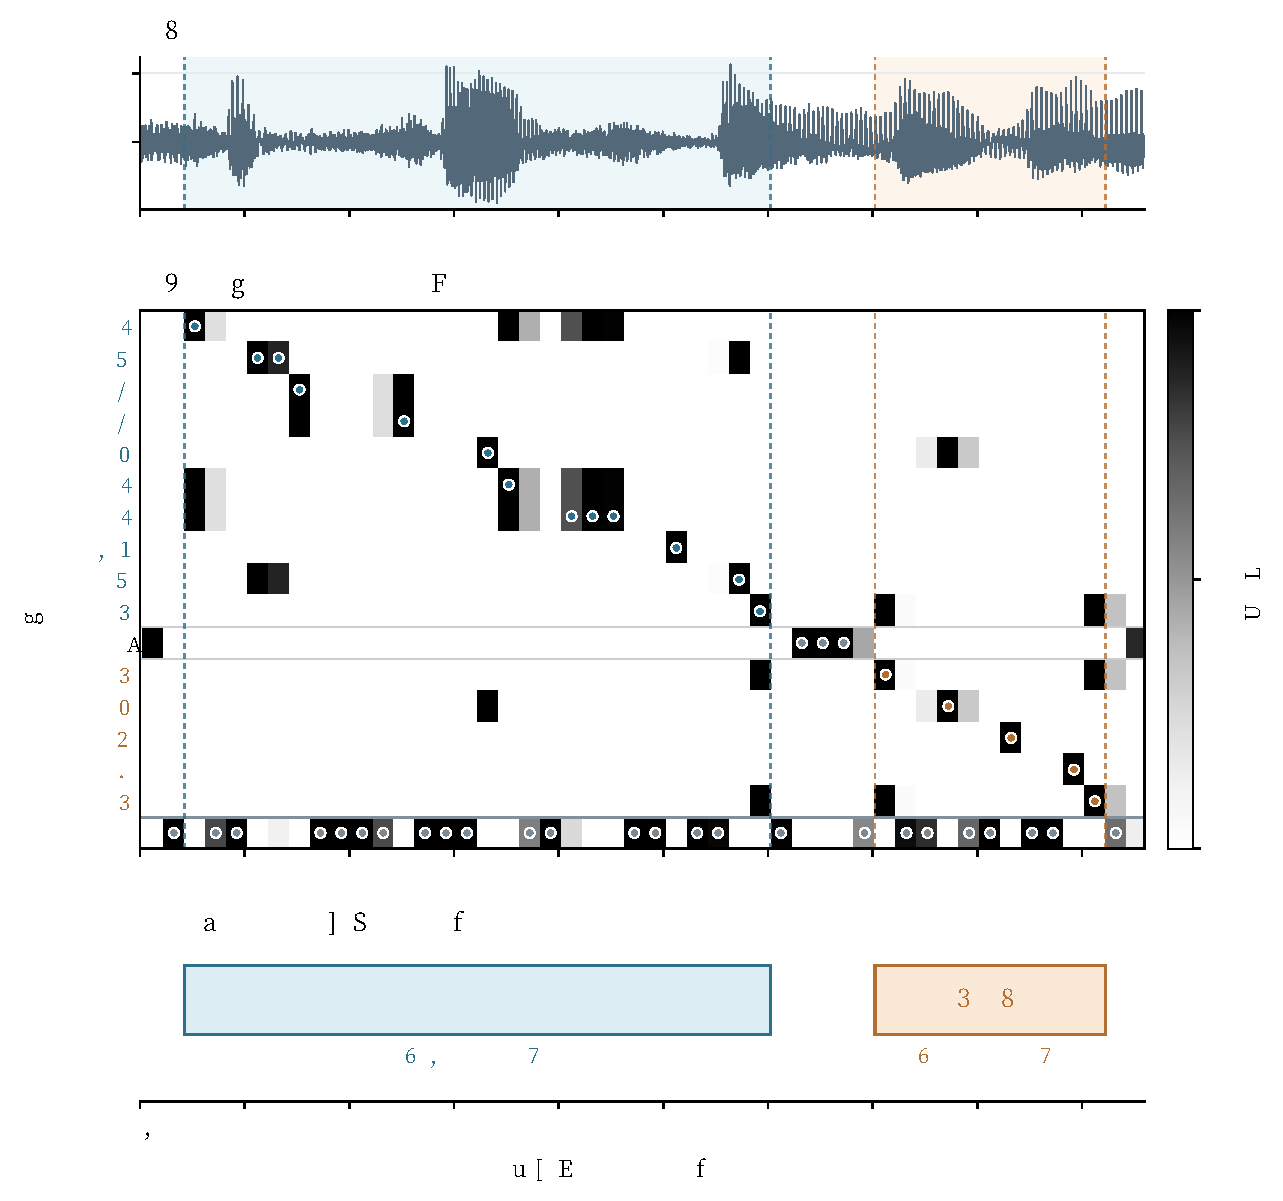
\includegraphics[width=0.96\textwidth]{figures/fig_5_4_ctc_word_alignment.pdf}
    \caption{基于CTC的文本与音频词级强制对齐实例。
    虚线标示估计的词起止时间，底部矩形表示候选词区间；时间均相对于视频起点。}
    \label{fig:p1_ctc_word_alignment}
\end{figure}

图中，相同字符因位于转写的不同位置而分别列出，其模型输出概率相同，
但最优路径按照目标字符顺序分配对应时刻。例如，\texttt{successful}
中的两个连续字母 \texttt{C} 对应不同的输出位置，并由空白状态分隔。
将属于同一原文词的文字字符时刻合并后，得到 \texttt{successful} 的候选区间为
$[1.842,\,2.402]\,\mathrm{s}$，\texttt{Legal} 的候选区间为
$[2.502,\,2.722]\,\mathrm{s}$，对应的词级置信度分别约为 $0.968$ 和 $0.998$。
该实例说明，词级时间区间由受转写约束的字符路径确定，无须按词数均分音频时长。
图中边界为模型估计结果，其时间准确性仍需结合后续质量核验判断。
